\section{\mAL\ and \ourL\ comparison}
	For a more clear comparison we show the execution, on both \mAL\ and \ourL, of the action instances sequence $\Delta_{c} = \distract{C}{A};\open{A};\peek{A}$, that leads to the desired goal, in the domain expressed in Example~\ref{ex:coin_box}.
	With this we want to give a graphical explanation of both the transition functions and state-space defined by the two languages. Each state in \mAL\ will be represented by a Kripke structure while in \ourL\ will be a \pos\ (expanded to its respective system of equations for clarity).
	%At the end of each state representation we also give some examples of entailed formulae.

	The observability relations of each action instance in $\Delta_c$ is expressed in the following Table:
	\begin{table}[H]
		\centering
		\begin{tabular}{||c||c|c|c||}
			\hhline{~|t:===:t|}
			\multicolumn{1}{c||}{}
			& \multicolumn{1}{c|}{\phantom{...}\distract{C}{A}\phantom{...}}
			& \multicolumn{1}{c|}{\phantom{..}\open{A}\phantom{..}}
			& \multicolumn{1}{c||}{\phantom{...}\peek{A}\phantom{...}}\\
			\hhline{|t:=::===:|}
			\multicolumn{1}{||c||}{$F_D$}
			& \multicolumn{1}{c|}{\agent A, \agent B, \agent C}
			& \multicolumn{1}{c|}{\agent A, \agent B}
			& \multicolumn{1}{c||}{\agent A}\\
			\hhline{||-||-|-|-||}
			\multicolumn{1}{||c||}{$P_D$}
			& \multicolumn{1}{c|}{-}
			& \multicolumn{1}{c|}{-}
			& \multicolumn{1}{c||}{\agent B}\\
			\hhline{||-||-|-|-||}
			\multicolumn{1}{||c||}{$O_D$}
			& \multicolumn{1}{c|}{-}
			& \multicolumn{1}{c|}{\agent C}
			& \multicolumn{1}{c||}{\agent C}\\
			\hhline{|b:=:b:===:b|}
		\end{tabular}
		\label{table-before-distract} 
		\caption{Observability relations of the actions instances in $\Delta_{c}$.}
	\end{table}%
%
The initial state, based on Example~\ref{ex:coin_box}, is defined by the conditions:
	\begin{enumerate}[label=]
		\item \initially{\C(\haskey{A})}
		\item \initially{\C(\neg \haskey{B})}
		\item \initially{\C(\neg \haskey{C})}
		\item \initially{\C(\neg \opened)}
		\item \initially{\C(\neg \bB{ag}{\head} \wedge \neg \bB{ag}{\neg \head})} for $\agent{ag} \in \bra{\agent{A}, \agent{B}, \agent{C}}$
		\item \initially{\C(\looking{ag})} for $\agent{ag} \in \bra{\agent{A}, \agent{B}, \agent{C}}$
		\item \initially{\neg \head}
	\end{enumerate}

Finally the goal that both the state in Figure~\ref{fig:appendix_peek} entail is expressed with the following formulae:
\begin{align*}
&\bB{A}{\neg \head} \wedge \bB{A}{(\bB{B}{(\bB{A}{\head}
		\vee \bB{A}{\neg \head})})}\\
&\bB{B}{(\bB{A}{\head}\vee \bB{A}{\neg \head})} \wedge
(\neg \bB{B}{\head \wedge \neg \bB{B}{\neg \head}})\\
&\bB{C}[\bigwedge_{\agent{AG} \in \bra{\agent A, \agent B, \agent C}}(\neg\bB{ag}{\head}
\wedge \neg\bB{ag}{\neg \head}) ]
%	\state{3}{z_0} &\models\,C_{\bra{\agent A, \agent B}}(\neg\bB{B}{\head} \wedge \neg \bB{B}{\head)}
\end{align*}
%
	\FloatBarrier
	\subsection*{The plan for Example~\ref{ex:coin_box}}
		\begin{figure}[H]
		\centering
		\hspace*{-3cm}
			\subfloat[The initial Kripke structure \state{0}{s_0}.]
			{%
				\scalebox{.8}%
				{%
					\raisebox{0.5cm}{
						

\tikzset{every picture/.style={line width=0.75pt}} %set default line width to 0.75pt        
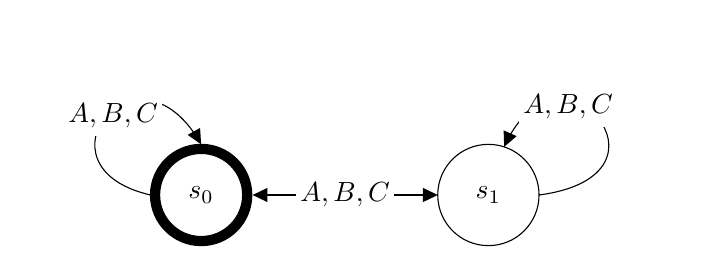
\begin{tikzpicture}[x=0.75pt,y=0.75pt,yscale=-0.8,xscale=0.8]
%uncomment if require: \path (0,150); %set diagram left start at 0, and has height of 150

%Shape: Circle [id:dp4325934269433842] 
\draw  [fill={rgb, 255:red, 0; green, 0; blue, 0 }  ,fill opacity=1 ] (216.5,93) .. controls (216.5,76.16) and (230.16,62.5) .. (247,62.5) .. controls (263.84,62.5) and (277.5,76.16) .. (277.5,93) .. controls (277.5,109.84) and (263.84,123.5) .. (247,123.5) .. controls (230.16,123.5) and (216.5,109.84) .. (216.5,93) -- cycle ;
%Shape: Circle [id:dp8959340303758652] 
\draw   (389.5,93) .. controls (389.5,76.16) and (403.16,62.5) .. (420,62.5) .. controls (436.84,62.5) and (450.5,76.16) .. (450.5,93) .. controls (450.5,109.84) and (436.84,123.5) .. (420,123.5) .. controls (403.16,123.5) and (389.5,109.84) .. (389.5,93) -- cycle ;
%Straight Lines [id:da6159546739572547] 
\draw    (280,93) -- (387.5,93) ;
\draw [shift={(389.5,93)}, rotate = 180] [fill={rgb, 255:red, 0; green, 0; blue, 0 }  ][line width=0.75]  [draw opacity=0] (8.93,-4.29) -- (0,0) -- (8.93,4.29) -- cycle    ;
\draw [shift={(278,93)}, rotate = 0] [fill={rgb, 255:red, 0; green, 0; blue, 0 }  ][line width=0.75]  [draw opacity=0] (8.93,-4.29) -- (0,0) -- (8.93,4.29) -- cycle    ;
%Curve Lines [id:da8452234444075793] 
\draw    (216.5,93) .. controls (142.87,76.08) and (207.84,-5.18) .. (246.42,61.48) ;
\draw [shift={(247,62.5)}, rotate = 240.66] [fill={rgb, 255:red, 0; green, 0; blue, 0 }  ][line width=0.75]  [draw opacity=0] (8.93,-4.29) -- (0,0) -- (8.93,4.29) -- cycle    ;

%Curve Lines [id:da8370233876099651] 
\draw    (450.5,93) .. controls (540.91,81.08) and (462.16,-7.43) .. (429.98,62.93) ;
\draw [shift={(429.5,64)}, rotate = 293.78] [fill={rgb, 255:red, 0; green, 0; blue, 0 }  ][line width=0.75]  [draw opacity=0] (8.93,-4.29) -- (0,0) -- (8.93,4.29) -- cycle    ;

%Shape: Circle [id:dp08152116050102409] 
\draw  [fill={rgb, 255:red, 255; green, 255; blue, 255 }  ,fill opacity=1 ] (222,93) .. controls (222,79.19) and (233.19,68) .. (247,68) .. controls (260.81,68) and (272,79.19) .. (272,93) .. controls (272,106.81) and (260.81,118) .. (247,118) .. controls (233.19,118) and (222,106.81) .. (222,93) -- cycle ;

% Text Node
\draw  [color={rgb, 255:red, 255; green, 255; blue, 255 }  ,draw opacity=1 ][fill={rgb, 255:red, 255; green, 255; blue, 255 }  ,fill opacity=1 ]  (304.75,81) -- (362.75,81) -- (362.75,105) -- (304.75,105) -- cycle  ;
\draw (333.75,93) node   {$\agent{A}, \agent{B}, \agent{C}$};
% Text Node
\draw (247,93) node   {$\defemph{s_0}$};
% Text Node
\draw (420,93) node   {$\defemph{s_1}$};
% Text Node
\draw  [color={rgb, 255:red, 255; green, 255; blue, 255 }  ,draw opacity=1 ][fill={rgb, 255:red, 255; green, 255; blue, 255 }  ,fill opacity=1 ]  (165,33) -- (223,33) -- (223,57) -- (165,57) -- cycle  ;
\draw (194,45) node   {$\agent{A}, \agent{B}, \agent{C}$};
% Text Node
\draw  [color={rgb, 255:red, 255; green, 255; blue, 255 }  ,draw opacity=1 ][fill={rgb, 255:red, 255; green, 255; blue, 255 }  ,fill opacity=1 ]  (439,28) -- (497,28) -- (497,52) -- (439,52) -- cycle  ;
\draw (468,40) node   {$\agent{A}, \agent{B}, \agent{C}$};

%\draw (340,160) node   {%
%	$\begin{aligned}
%	\interp{0}{s_0}&=\bra{\looking {AG}, \haskey A}\\
%	\interp{0}{s_1}&=\bra{\looking {AG}, \haskey{A}, \head}
%	\end{aligned}$
%	\hspace*{0.2cm}where \agent{ag} $\in$ \bra{\agent{a}, \agent{b}, \agent{c}}.};

\end{tikzpicture}


					}%
				}%
				\label{subfig-kripke:appendix_initial}
			}%
		\hspace*{.5cm}
			\subfloat[The initial \pos\ \poss{u}.]
			{% 
				\scalebox{0.95}%
				{%
					\raisebox{1.5cm}{
						
$\begin{cases}
 \poss u &= \bra{(\agentSlide{ag},\bra{\poss{u}, \poss{u^\prime}}),\\
 	&\text{~~~~~}\ttSlide{look(\agentSlide{ag})}, \ttSlide{key(\agentSlide{A})}, \ttSlide{heads}}\\
 \poss u^\prime &= \bra{(\agentSlide{ag},\bra{\poss{u}, \poss{u^\prime}}),\\
 	&\text{~~~~~}\ttSlide{look(\agentSlide{ag})}, \ttSlide{key(\agentSlide{A})}}
\end{cases}$

					}%
				}%
				\label{subfig-poss:appendix_initial}%
			}
			\caption{The initial state.}
			\label{fig:appendix_initial}
		\end{figure}%
%
		\begin{figure}[H]
			\centering
			\hspace*{-3cm}
			\subfloat[The Kripke stucture \state{1}{p_0}, obtained after the execution of \distract{C}{A}
			in \state{0}{s_0} (Figure~\ref{subfig-kripke:appendix_initial}).]
			{%
				\scalebox{.8}%
				{%
					\raisebox{0.5cm}{
						\input{img/distract_state_kripke}
					}%
				}%
				\label{subfig-kripke:appendix_distract}
			}%
			\hspace*{.5cm}
			\subfloat[\Pos\ \poss{v}, obtained after the execution of \distract{C}{A} in
			\poss{u} (Figure~\ref{subfig-poss:appendix_initial}).]
			{%
				\scalebox{0.95}%
				{%
					\raisebox{1.5cm}{
						$
\begin{aligned}
	&\begin{cases}
		\poss{v}&= \bra{
	     	(\agent{ag},\bra{\poss{v}, \poss{v^\prime}}),	\looking{a},
	     	\looking{b},
	     	\haskey{a}%
		}\\
			\poss{v}^\prime&= \bra{
	    	(\agent{ag},\bra{\poss{v}, \poss{v^\prime}}),
	    	\looking{a},
	    	\looking{b},
	    	\haskey{a},
	    	\head%
		}\\
	\end{cases}\\
	&\text{where }  \agent{ag}  \in \bra{\agent{A}, \agent{B}, \agent{C}}
\end{aligned}
$



					}%
				}%
				\label{subfig-poss:appendix_distract}%
			}
			\caption{Execution of \distract{C}{A}.}
			\label{fig:appendix_distract}
		\end{figure}%
%
		\begin{figure}[H]
			\centering
			\hspace*{-4cm}
			\subfloat[The Kripke stucture \state{2}{q_0}, obtained after the execution of \open{A}
			in \state{1}{p_0} (Figure~\ref{subfig-kripke:appendix_distract}).]
			{%
				\scalebox{.7}%
				{%
					\raisebox{0.0cm}{
						

\tikzset{every picture/.style={line width=0.75pt}} %set default line width to 0.75pt        

\begin{tikzpicture}[x=0.75pt,y=0.75pt,yscale=-1,xscale=1]
%uncomment if require: \path (0,371); %set diagram left start at 0, and has height of 371

%Shape: Circle [id:dp4325934269433842] 
\draw   (171.5,287) .. controls (171.5,270.16) and (185.16,256.5) .. (202,256.5) .. controls (218.84,256.5) and (232.5,270.16) .. (232.5,287) .. controls (232.5,303.84) and (218.84,317.5) .. (202,317.5) .. controls (185.16,317.5) and (171.5,303.84) .. (171.5,287) -- cycle ;
%Shape: Circle [id:dp8959340303758652] 
\draw   (344.5,287) .. controls (344.5,270.16) and (358.16,256.5) .. (375,256.5) .. controls (391.84,256.5) and (405.5,270.16) .. (405.5,287) .. controls (405.5,303.84) and (391.84,317.5) .. (375,317.5) .. controls (358.16,317.5) and (344.5,303.84) .. (344.5,287) -- cycle ;
%Straight Lines [id:da6159546739572547] 
\draw    (235,287) -- (342.5,287) ;
\draw [shift={(344.5,287)}, rotate = 180] [fill={rgb, 255:red, 0; green, 0; blue, 0 }  ][line width=0.75]  [draw opacity=0] (8.93,-4.29) -- (0,0) -- (8.93,4.29) -- cycle    ;
\draw [shift={(233,287)}, rotate = 0] [fill={rgb, 255:red, 0; green, 0; blue, 0 }  ][line width=0.75]  [draw opacity=0] (8.93,-4.29) -- (0,0) -- (8.93,4.29) -- cycle    ;
%Curve Lines [id:da8452234444075793] 
\draw    (171.5,287) .. controls (72.5,271.08) and (154.67,188.33) .. (193.42,254.98) ;
\draw [shift={(194,256)}, rotate = 240.66] [fill={rgb, 255:red, 0; green, 0; blue, 0 }  ][line width=0.75]  [draw opacity=0] (8.93,-4.29) -- (0,0) -- (8.93,4.29) -- cycle    ;

%Curve Lines [id:da8370233876099651] 
\draw    (405.5,287) .. controls (495.91,275.08) and (417.16,186.57) .. (384.98,256.93) ;
\draw [shift={(384.5,258)}, rotate = 293.78] [fill={rgb, 255:red, 0; green, 0; blue, 0 }  ][line width=0.75]  [draw opacity=0] (8.93,-4.29) -- (0,0) -- (8.93,4.29) -- cycle    ;

%Shape: Circle [id:dp7932635156571649] 
\draw  [fill={rgb, 255:red, 0; green, 0; blue, 0 }  ,fill opacity=1 ] (172.5,104) .. controls (172.5,87.16) and (186.16,73.5) .. (203,73.5) .. controls (219.84,73.5) and (233.5,87.16) .. (233.5,104) .. controls (233.5,120.84) and (219.84,134.5) .. (203,134.5) .. controls (186.16,134.5) and (172.5,120.84) .. (172.5,104) -- cycle ;
%Shape: Circle [id:dp6105058367437692] 
\draw   (345.5,104) .. controls (345.5,87.16) and (359.16,73.5) .. (376,73.5) .. controls (392.84,73.5) and (406.5,87.16) .. (406.5,104) .. controls (406.5,120.84) and (392.84,134.5) .. (376,134.5) .. controls (359.16,134.5) and (345.5,120.84) .. (345.5,104) -- cycle ;
%Straight Lines [id:da9340669325180512] 
\draw    (236,104) -- (343.5,104) ;
\draw [shift={(345.5,104)}, rotate = 180] [fill={rgb, 255:red, 0; green, 0; blue, 0 }  ][line width=0.75]  [draw opacity=0] (8.93,-4.29) -- (0,0) -- (8.93,4.29) -- cycle    ;
\draw [shift={(234,104)}, rotate = 0] [fill={rgb, 255:red, 0; green, 0; blue, 0 }  ][line width=0.75]  [draw opacity=0] (8.93,-4.29) -- (0,0) -- (8.93,4.29) -- cycle    ;
%Curve Lines [id:da4572197115547698] 
\draw    (172.5,104) .. controls (98.87,87.08) and (163.84,5.82) .. (202.42,72.48) ;
\draw [shift={(203,73.5)}, rotate = 240.66] [fill={rgb, 255:red, 0; green, 0; blue, 0 }  ][line width=0.75]  [draw opacity=0] (8.93,-4.29) -- (0,0) -- (8.93,4.29) -- cycle    ;

%Curve Lines [id:da9119172492888147] 
\draw    (406.5,104) .. controls (496.91,92.08) and (418.16,3.57) .. (385.98,73.93) ;
\draw [shift={(385.5,75)}, rotate = 293.78] [fill={rgb, 255:red, 0; green, 0; blue, 0 }  ][line width=0.75]  [draw opacity=0] (8.93,-4.29) -- (0,0) -- (8.93,4.29) -- cycle    ;

%Shape: Circle [id:dp47196260233615805] 
\draw  [fill={rgb, 255:red, 255; green, 255; blue, 255 }  ,fill opacity=1 ] (178,104) .. controls (178,90.19) and (189.19,79) .. (203,79) .. controls (216.81,79) and (228,90.19) .. (228,104) .. controls (228,117.81) and (216.81,129) .. (203,129) .. controls (189.19,129) and (178,117.81) .. (178,104) -- cycle ;
%Straight Lines [id:da04653031760639226] 
\draw    (222.75,125.5) -- (357.09,260.58) ;
\draw [shift={(358.5,262)}, rotate = 225.16] [fill={rgb, 255:red, 0; green, 0; blue, 0 }  ][line width=0.75]  [draw opacity=0] (8.93,-4.29) -- (0,0) -- (8.93,4.29) -- cycle    ;

%Straight Lines [id:da7004759142531133] 
\draw    (362.13,131.25) -- (216.63,258.93) ;
\draw [shift={(215.13,260.25)}, rotate = 318.73] [fill={rgb, 255:red, 0; green, 0; blue, 0 }  ][line width=0.75]  [draw opacity=0] (8.93,-4.29) -- (0,0) -- (8.93,4.29) -- cycle    ;

%Straight Lines [id:da7971203391650094] 
\draw    (203,134.5) -- (202.02,254.5) ;
\draw [shift={(202,256.5)}, rotate = 270.47] [fill={rgb, 255:red, 0; green, 0; blue, 0 }  ][line width=0.75]  [draw opacity=0] (8.93,-4.29) -- (0,0) -- (8.93,4.29) -- cycle    ;

%Straight Lines [id:da21593783196193417] 
\draw    (376,134.5) -- (375.02,254.5) ;
\draw [shift={(375,256.5)}, rotate = 270.47] [fill={rgb, 255:red, 0; green, 0; blue, 0 }  ][line width=0.75]  [draw opacity=0] (8.93,-4.29) -- (0,0) -- (8.93,4.29) -- cycle    ;


% Text Node
\draw  [color={rgb, 255:red, 255; green, 255; blue, 255 }  ,draw opacity=1 ][fill={rgb, 255:red, 255; green, 255; blue, 255 }  ,fill opacity=1 ]  (259.75,275) -- (317.75,275) -- (317.75,299) -- (259.75,299) -- cycle  ;
\draw (288.75,287) node   {\{$\agentSlide{A},\agentSlide{B},\agentSlide{C}$\}};
% Text Node
\draw (202,287) node   {\defemph{p_{0}}};
% Text Node
\draw (375,287) node   {\defemph{p_{1}}};
% Text Node
\draw  [color={rgb, 255:red, 255; green, 255; blue, 255 }  ,draw opacity=1 ][fill={rgb, 255:red, 255; green, 255; blue, 255 }  ,fill opacity=1 ]  (120,227) -- (178,227) -- (178,251) -- (120,251) -- cycle  ;
\draw (149,239) node   {\{$\agentSlide{A}, \agentSlide{B},\agentSlide{C}$\}};
% Text Node
\draw  [color={rgb, 255:red, 255; green, 255; blue, 255 }  ,draw opacity=1 ][fill={rgb, 255:red, 255; green, 255; blue, 255 }  ,fill opacity=1 ]  (394,222) -- (452,222) -- (452,246) -- (394,246) -- cycle  ;
\draw (423,234) node   {\{$\agentSlide{A},\agentSlide{B},\agentSlide{C}$\}};
% Text Node
\draw  [color={rgb, 255:red, 255; green, 255; blue, 255 }  ,draw opacity=1 ][fill={rgb, 255:red, 255; green, 255; blue, 255 }  ,fill opacity=1 ]  (270.25,92) -- (309.25,92) -- (309.25,116) -- (270.25,116) -- cycle  ;
\draw (289.75,104) node   {\{$\agentSlide{A},\agentSlide{B}$\}};
% Text Node
\draw (203,104) node   {\defemph{q_{0}}};
% Text Node
\draw (376,104) node   {\defemph{q_{1}}};
% Text Node
\draw  [color={rgb, 255:red, 255; green, 255; blue, 255 }  ,draw opacity=1 ][fill={rgb, 255:red, 255; green, 255; blue, 255 }  ,fill opacity=1 ]  (130.5,44) -- (169.5,44) -- (169.5,68) -- (130.5,68) -- cycle  ;
\draw (150,56) node   {\{$\agentSlide{A},\agentSlide{B}$\}};
% Text Node
\draw  [color={rgb, 255:red, 255; green, 255; blue, 255 }  ,draw opacity=1 ][fill={rgb, 255:red, 255; green, 255; blue, 255 }  ,fill opacity=1 ]  (405.5,39) -- (444.5,39) -- (444.5,63) -- (405.5,63) -- cycle  ;
\draw (425,51) node   {\{$\agentSlide{A},\agentSlide{B}$\}};
% Text Node
\draw  [color={rgb, 255:red, 255; green, 255; blue, 255 }  ,draw opacity=1 ][fill={rgb, 255:red, 255; green, 255; blue, 255 }  ,fill opacity=1 ]  (188,174) -- (208,174) -- (208,198) -- (188,198) -- cycle  ;
\draw (198,186) node   {\{$\agentSlide{C}$\}};
% Text Node
\draw  [color={rgb, 255:red, 255; green, 255; blue, 255 }  ,draw opacity=1 ][fill={rgb, 255:red, 255; green, 255; blue, 255 }  ,fill opacity=1 ]  (234,140) -- (254,140) -- (254,164) -- (234,164) -- cycle  ;
\draw (244,152) node   {\{$\agentSlide{C}$\}};
% Text Node
\draw  [color={rgb, 255:red, 255; green, 255; blue, 255 }  ,draw opacity=1 ][fill={rgb, 255:red, 255; green, 255; blue, 255 }  ,fill opacity=1 ]  (327,140) -- (347,140) -- (347,164) -- (327,164) -- cycle  ;
\draw (337,152) node   {\{$\agentSlide{C}$\}};
% Text Node
\draw  [color={rgb, 255:red, 255; green, 255; blue, 255 }  ,draw opacity=1 ][fill={rgb, 255:red, 255; green, 255; blue, 255 }  ,fill opacity=1 ]  (366,175) -- (386,175) -- (386,199) -- (366,199) -- cycle  ;
\draw (376,187) node   {\{$\agentSlide{C}$\}};

\draw (310,380) node   {
							$\begin{aligned}
							\interp{2}{q_0}&=\bra{\ttSlide{look(\agentSlide{ag})}, \ttSlide{key(\agentSlide{A})}, \ttSlide{opened}, \ttSlide{heads}}\\
							\interp{2}{q_1}&=\bra{\ttSlide{look(\agentSlide{ag})}, \ttSlide{key(\agentSlide{A})}, \ttSlide{opened}}\\
							\interp{2}{p_0}&=\interp{1}{p_0}\\
							\interp{2}{p_1}&=\interp{1}{p_1}
						\end{aligned}$};

\end{tikzpicture}


					}%
				}%
				\label{subfig-kripke:appendix_open}
			}%
			\hspace*{.5cm}
			\subfloat[\Pos\ \poss{w}, obtained after the execution of \open{A} in
			\poss{v} (Figure~\ref{subfig-poss:appendix_distract}).]
			{%
				\scalebox{0.95}%
				{%
					\raisebox{3.6cm}{
						$\begin{aligned}
  &\begin{cases}
    \poss{w}&= \bra{
      (\agentSlide{ag},\bra{\poss{w}, \poss{w^\prime}}),
      (\agentSlide{c},\bra{\poss{v}, \poss{v^\prime}}),\\
      &\text{~~~~~}\ttSlide{look(\agentSlide{ag})},
      \ttSlide{key(\agentSlide{A})},
      \ttSlide{opened}, \ttSlide{heads}}\\
    \poss{w^\prime} &=\bra{
      (\agentSlide{ag},\bra{\poss{w}, \poss{w^\prime}}),
      (\agentSlide{c},\bra{\poss{v}, \poss{v^\prime}}),\\
      &\text{~~~~~}\ttSlide{look(\agentSlide{ag})}, \ttSlide{key(\agentSlide{A})}, \ttSlide{opened}}
   \end{cases}\\
  &\text{where } \poss{v},
            \poss{v^\prime}, \text{ are defined as before}.
\end{aligned}$

					}%
				}%
				\label{subfig-poss:appendix_open}%
			}
			\caption{Execution of \open{A}.}
			\label{fig:appendix_open}
		\end{figure}%
%
		\begin{figure}[H]
			%\centering
			\hspace*{-4cm}
			\subfloat[The Kripke structure \state{3}{q_0}, obtained after the execution of \peek{A} in \state{2}{q_0}.]
			{%
				\scalebox{.7}%
				{%
					\raisebox{0.0cm}{
						\input{img/peek_state_kripke}
					}%
				}%
				\label{subfig-kripke:appendix_peek}
			}%
			\hspace*{.5cm}
			\subfloat[\Pos\ \poss{z}, obtained after the execution of \peek{A} in
			\poss{w} (Figure~\ref{subfig-poss:appendix_open}).]
			{% 
				\scalebox{0.95}%
				{%
					\raisebox{3.6cm}{
						$\begin{aligned}
&\begin{cases}
\poss{z} &= \bra{
	(\agentSlide{A},\bra{\poss{z}}), (\agentSlide{B}, \bra{\poss{z}, \poss{z^\prime}}) (\agentSlide{C}, \bra{\poss{v}, \poss{v^\prime}}),\\
	&\text{~~~~~}\ttSlide{look(\agentSlide{ag})},
	\ttSlide{key(\agentSlide{A})},
	\ttSlide{opened},
	\ttSlide{heads}}\\
\poss{z^\prime} &= \bra{
	(\agentSlide{A},\bra{\poss{z^\prime}}), (\agentSlide{B}, \bra{\poss{z}, \poss{z^\prime}}) (\agentSlide{C}, \bra{\poss{v}, \poss{v^\prime}}),\\
	&\text{~~~~~}\ttSlide{look(\agentSlide{ag})},
	\ttSlide{key(\agentSlide{A})},
	\ttSlide{opened},}
\end{cases}\\
&\text{where the \posS\ \poss{v}, \poss{v^\prime} are defined as before.}
\end{aligned}$



					}%
				}%
				\label{subfig-poss:appendix_peek}%
			}
			\caption{Execution of \peek{A}.}
			\label{fig:appendix_peek}
		\end{figure}%
%	
%		Both the state in Figure~\ref{fig:appendix_peek} entail the desired goal that is expressed with the following formulae:
%		\begin{align*}
%			&\bB{A}{\neg \head} \wedge \bB{A}{(\bB{B}{(\bB{A}{\head}
%				\vee \bB{A}{\neg \head})})}\\
%			&\bB{B}{(\bB{A}{\head}\vee \bB{A}{\neg \head})} \wedge
%			(\neg \bB{B}{\head \wedge \neg \bB{B}{\neg \head}})\\
%			&\bB{C}[\bigwedge_{\agent{AG} \in \bra{\agent A, \agent B, \agent C}}(\neg\bB{ag}{\head}
%			\wedge \neg\bB{ag}{\neg \head}) ]
%		%	\state{3}{z_0} &\models\,C_{\bra{\agent A, \agent B}}(\neg\bB{B}{\head} \wedge \neg \bB{B}{\head)}
%		\end{align*}
%		\begin{align*}
%			\state{3}{z_0} &\models \bB{A}{\neg \head} \wedge \bB{A}{(\bB{B}{(\bB{A}{\head}
%					\vee \bB{A}{\neg \head})})}\\
%			\state{3}{z_0} &\models \bB{B}{(\bB{A}{\head}\vee \bB{A}{\neg \head})} \wedge
%			(\neg \bB{B}{\head \wedge \neg \bB{B}{\neg \head}})\\
%			\state{3}{z_0} &\models \bB{C}[\bigwedge_{\agent{AG} \in \bra{\agent A, \agent B, \agent C}}(\neg\bB{ag}{\head}
%			\wedge \neg\bB{ag}{\neg \head}) ]
%		%	\state{3}{z_0} &\models\,C_{\bra{\agent A, \agent B}}(\neg\bB{B}{\head} \wedge \neg \bB{B}{\head)}
%		\end{align*}